\documentclass{article}
\usepackage[utf8]{inputenc}
\usepackage{listings}
\usepackage{graphicx}
\usepackage{float}
\usepackage{xcolor}
\usepackage{geometry}
\usepackage{CJKutf8}
\usepackage{amsmath}
\usepackage{amssymb}

\geometry{a4paper,scale=0.8}
\lstset{
    basicstyle          =   \sffamily,        
    keywordstyle        =   \bfseries,         
    commentstyle        =   \rmfamily\itshape, 
    stringstyle         =   \ttfamily, 
    flexiblecolumns,               
    numbers             =   left,  
    showspaces          =   false, 
    showstringspaces    =   false,
    captionpos          =   t,     
    frame               =   lrtb, 
}

\lstdefinestyle{Python}{
    language        =   Python, % 语言选Python
    basicstyle      =   \zihao{-5}\ttfamily,
    numberstyle     =   \zihao{-5}\ttfamily,
    keywordstyle    =   \color{blue},
    keywordstyle    =   [2] \color{teal},
    stringstyle     =   \color{magenta},
    commentstyle    =   \color{red}\ttfamily,
    breaklines      =   true,  
    columns         =   fixed,  
    basewidth       =   0.5em,
}

\title{\bf\Large  概率论与数理统计 第10次作业}
%%%%%%%%%%%%%%%%%%%%%%%%%%%%%%%%%%%%%%
%% DON'T forget to change this part %%
\author{\bf Name: 宋昊原 \qquad Student ID: 2022010755}
%%%%%%%%%%%%%%%%%%%%%%%%%%%%%%%%%%%%%%

\begin{document}
\begin{CJK}{UTF8}{gbsn}
\maketitle
\section{简单随机抽样}
\subsection{}
$$ E(\hat{\sigma}^{2})=\frac{1}{n}\sum\limits_{i=1}^{n}(E(X_{i}^{2})-2E(X_{i}\bar{X})+E(\bar{X}^{2}))$$
考虑到对称性,有
$$ E(\hat{\sigma}^{2})=E(X_{1}^{2})-2E(X_{1}\bar{X})+E(\bar{X}^{2})$$
$$ =E(X_{1}^{2})-\frac{2}{n}E(X_{1}^{2})-\frac{2(n-1)}{n}E(X_{1}X_{2})+\frac{1}{n}E(X_{1}^{2})+\frac{n-1}{n}E(X_{1}X_{2})$$
$$ =\frac{n-1}{n}E(X_{1}^{2})-\frac{n-1}{n}E(X_{1}X_{2})$$
其中
$$ E(X_{1}^{2})=\mu^{2}+\sigma^{2}$$
$$ E(X_{1}X_{2})=\frac{1}{N(N-1)}\sum\limits_{i\neq j}x_{i}x_{j}$$
$$ =\frac{1}{N(N-1)}((\sum\limits_{i}x_{i})^{2}-\sum\limits_{i}x_{i}^{2})$$
$$ =\frac{1}{N(N-1)}(N^{2}\mu^{2}-N(\mu^{2}+\sigma^{2}))=\mu^{2}-\frac{1}{N-1}\sigma^{2}$$
故
$$ E(\hat{\sigma}^{2})=\sigma^{2}\frac{n-1}{n}\frac{N}{N-1}$$
\subsection{}
作业9-3计算过
$$ Var(\bar{X})=\sigma^{2}\frac{1}{n}\frac{N-n}{N-1}$$
故
$$ Var(\bar{X})=\frac{N-n}{N(n-1)}E(\hat{\sigma}^{2})$$
当$N,n$都已知时
$$ \frac{N-n}{N(n-1)}\hat{\sigma}^{2}$$
是$Var(\bar{X})$的一个无偏估计.
\section{Poisson分布的估计}
\subsection{}
Poisson分布为
$$ P(X=k)=\frac{\lambda^{k}}{k!}e^{-\lambda}$$
首先证明$\hat{\theta}$是无偏估计
$$E(\hat{\theta}(X))=\sum\limits_{k=0}^{\infty}\frac{\lambda^{2k}}{(2k)!}e^{-\lambda}-\sum\limits_{k=0}^{\infty}\frac{\lambda^{2k+1}}{(2k+1)!}e^{-\lambda}$$
$$=e^{-\lambda}\sum\limits_{k=0}^{\infty}\frac{\lambda^{k}(-1)^{k}}{k!}e^{-\lambda}=e^{-\lambda}e^{-\lambda}=e^{-2\lambda}$$
再证明唯一性,此时样本容量为1,故估计量只能是$X$的函数,若此函数是无偏估计,则
$$ E(\hat{\theta}(X))=\sum\limits_{k=0}^{\infty}\frac{\lambda^{k}}{k!}e^{-\lambda}\hat{\theta}(k)=e^{-2\lambda}$$
故
$$\sum\limits_{k=0}^{\infty}\frac{\lambda^{k}}{k!}\hat{\theta}(k)=e^{-\lambda}$$
已知
$$\sum\limits_{k=0}^{\infty}\frac{\lambda^{k}}{k!}(-1)^{k}=e^{-\lambda}$$
即
$$\forall\lambda>0,\ \sum\limits_{k=0}^{\infty}\frac{\lambda^{k}}{k!}\hat{\theta}(k)=\sum\limits_{k=0}^{\infty}\frac{\lambda^{k}}{k!}(-1)^{k}$$
这两个幂级数收敛于同一函数必须要求其系数分别相等,即
$$ \hat{\theta}(X)=(-1)^{X}$$
是唯一的无偏估计.
\subsection{}
上述估计不合理,由于$\lambda>0$,有
$$ 0<e^{-2\lambda}<1$$
故上述估计给出的是完全荒谬的结果.
\\\\
要给出合理的估计,可以采用极大似然估计,似然函数为
$$ L(\theta)=\frac{\lambda^{X}}{X!}e^{-\lambda}$$
故
$$ \frac{dL}{d\theta}=\frac{X\lambda^{X-1}e^{-\lambda}-\lambda^{X}e^{-\lambda}}{X!}$$
令此值为0,则有
$$ \lambda=X$$
这确实是最大值.
\\实际上,由于$E(X)=\lambda$,这和矩估计给出相同的结果.
\section{均匀总体的估计}
\subsection{}
考虑最小值、最大值的CDF
$$ F_{1}(x)=1-\frac{(\theta-x)^{n}}{\theta^{n}}$$
$$ F_{n}(x)=\frac{x^{n}}{\theta^{n}}$$
则PDF
$$ f_{1}(x)=\frac{n(\theta-x)^{n-1}}{\theta^{n}}$$
$$ f_{n}(x)=\frac{nx^{n-1}}{\theta^{n}}$$
故
$$ E(\hat{\theta_{1}})=\int_{0}^{\theta}\frac{nx(\theta-x)^{n-1}}{\theta^{n}}dx+\int_{0}^{\theta}\frac{nx^{n}}{\theta^{n}}dx$$
$$ =\int_{0}^{\theta}\frac{n(\theta-x)x^{n-1}}{\theta^{n}}dx+\int_{0}^{\theta}\frac{nx^{n}}{\theta^{n}}dx$$
$$=\int_{0}^{\theta}\frac{nx^{n-1}}{\theta^{n-1}}dx=\theta$$
故$\hat{\theta_{1}}$是$\theta$的无偏估计.
\subsection{}
考虑最小值$X_{min}$的期望
$$ E(X_{min})=\int_{0}^{\theta}\frac{nx(\theta-x)^{n-1}}{\theta^{n}}dx$$
$$ =\int_{0}^{\theta}\frac{n(\theta-x)x^{n-1}}{\theta^{n}}dx=\int_{0}^{\theta}\frac{n\theta x^{n-1}-nx^{n}}{\theta^{n}}dx$$
$$ =\theta-\frac{n}{n+1}\theta=\frac{\theta}{n+1}$$
于是取
$$ c_{n}=n+1$$
则
$$\hat{\theta_{2}}=(n+1)X_{min}$$
是$\theta$的无偏估计.
\subsection{}
考虑$X_{min},X_{max}$的联合累积分布函数
$$F(x_{m},x_{M})=P(X_{min}\leq x_{m}\land X_{max}\leq x_{M})$$
$$ =P(X_{max}\leq x_{M})-P(X_{min}> x_{m}\land X_{max}\leq x_{M})$$
$$ =(\frac{x_{M}}{\theta})^{n}-(\frac{x_{M}-x_{m}}{\theta})^{n}$$
于是其联合PDF为
$$f(x_{m},x_{M})=\frac{\partial^{2}}{\partial x_{m}\partial x_{M}}F(x_{m},x_{M})=\frac{n(n-1)(x_{M}-x_{m})^{n-2}}{\theta^{n}}$$
$0\leq x\leq\theta$时
$$\hat{f_{1}}(x)=\int_{0}^{\frac{x}{2}}f(\xi,x-\xi)d\xi=\int_{0}^{\frac{x}{2}}\frac{n(n-1)(x-2\xi)^{n-2}}{\theta^{n}}d\xi$$
$$=-\frac{1}{2}\int_{0}^{\frac{x}{2}}\frac{n(n-1)(x-2\xi)^{n-2}}{\theta^{n}}d(x-2\xi)$$
$$=\frac{nx^{n-1}}{2\theta^{n}}$$
$\theta<x\leq 2\theta$时
$$\hat{f_{1}}(x)=\int_{x-\theta}^{\frac{x}{2}}f(\xi,x-\xi)d\xi=\int_{x-\theta}^{\frac{x}{2}}\frac{n(n-1)(x-2\xi)^{n-2}}{\theta^{n}}d\xi$$
$$ =\frac{n(2\theta-x)^{n-1}}{2\theta^{n}}$$
故
$$Var(\hat{\theta_{1}})=E(\hat{\theta_{1}}^{2})-\theta^{2}$$
$$=\int_{0}^{\theta}\frac{nx^{n+1}}{2\theta^{n}}dx+\int_{\theta}^{2\theta}\frac{n(2\theta-x)^{n-1}x^{2}}{2\theta^{n}}dx-\theta^{2}$$
$$=\frac{n\theta^{2}}{2(n+2)}+\int_{0}^{\theta}\frac{nx^{n-1}(2\theta-x)^{2}}{2\theta^{n}}dx-\theta^{2}$$
$$=\frac{n\theta^{2}}{n+2}-\frac{2n\theta^{2}}{n+1}+2\theta^{2}-\theta^{2}$$
$$=\frac{2\theta^{2}}{(n+1)(n+2)}$$
而
$$Var(\hat{\theta_{2}})=(n+1)^{2}Var(X_{min})$$
$$=(n+1)^{2}E(X_{min}^{2})-\theta^{2}$$
$$=(n+1)^{2}\int_{0}^{\theta}\frac{n(\theta-x)^{n-1}x^{2}}{\theta^{n}}dx-\theta^{2}$$
$$=\frac{n\theta^{2}}{n+2}$$
$$Var(\hat{\theta_{3}})=4Var(\bar{X})=\frac{\theta^{2}}{3n}$$
$$Var(\hat{\theta_{4}})=\frac{(n+1)^{2}}{n^{2}}E(X_{max}^{2})-\theta^{2}$$
$$=\frac{(n+1)^{2}}{n^{2}}\int_{0}^{\theta}\frac{nx^{n+1}}{\theta^{n}}dx-\theta^{2}$$
$$=\frac{\theta^{2}}{n(n+2)}$$
在$n\to\infty$的渐近条件下有
$$Var(\hat{\theta_{2}})>>Var(\hat{\theta_{3}})>>Var(\hat{\theta_{1}})>Var(\hat{\theta_{4}})$$
这说明,在估计中引入较大的次序统计量的权重越大,估计的方差就越小.
\section{加权平均估计}
\subsection{}
$$ E(\sum\limits_{i=1}^{n}c_{i}X_{i})=\sum\limits_{i=1}^{n}c_{i}E(X_{i})=\theta\sum\limits_{i=1}^{n}c_{i}$$
故
$$ E(\sum\limits_{i=1}^{n}c_{i}X_{i})=\theta\Leftrightarrow\sum\limits_{i=1}^{n}c_{i}=1$$
\subsection{}
设总体方差为$\sigma^{2}$
$$E((\sum\limits_{i=1}^{n}c_{i}X_{i})^{2})=(\theta^{2}+\sigma^{2})\sum\limits_{i=1}^{n}c_{i}^{2}+\theta^{2}\sum\limits_{i\neq j}c_{i}c_{j}$$
$$ =\theta^{2}(\sum\limits_{i=1}^{n}c_{i})^{2}+\sigma^{2}\sum\limits_{i=1}^{n}c_{i}^{2}$$
$$ =\theta^{2}+\sigma^{2}\sum\limits_{i=1}^{n}c_{i}^{2}$$
$$ \geq\theta^{2}+\sigma^{2}\frac{\sum\limits_{i=1}^{n}c_{i}}{n}$$
$$ =\theta^{2}+\frac{1}{n}\sigma^{2}$$
上式取等当且仅当
$$ c_{1}=...=c_{n}=\frac{1}{n}$$
\section{正态估计的均方误差}
由于
$$ \frac{(n-1)S^{2}}{\sigma^{2}}\sim\chi^{2}(n-1)$$
可知
$$ Var(S^{2})=\frac{\sigma^{4}}{(n-1)^{2}}Var(\chi^{2}(n-1))=\frac{2\sigma^{4}}{n-1}$$
而
$$ Var(m_{2})=\frac{(n-1)^{2}}{n^{2}}Var(S^{2})=\frac{2(n-1)\sigma^{4}}{n^{2}}$$
$$ E((m_{2}-\sigma^{2})^{2})=Var(m_{2}-\sigma^{2})+E^{2}(m_{2}-\sigma^{2})=\frac{2(n-1)\sigma^{4}}{n^{2}}+\frac{\sigma^{4}}{n^{2}}=\frac{(2n-1)\sigma^{4}}{n^{2}}$$
而
$$ E((S^{2}-\sigma^{2})^{2})=Var(S^{2})=\frac{2\sigma^{4}}{n-1}=\frac{(2n-1)\sigma^{4}}{n^{2}-\frac{3}{2}n+\frac{1}{2}}$$
故
$$ E((S^{2}-\sigma^{2})^{2})>E((m_{2}-\sigma^{2})^{2})$$
\section{正态分布与t分布}
分母
$$ \frac{X_{3}^{2}+X_{4}^{2}}{4}\sim\chi^{2}(2)$$
分子
$$ \frac{X_{1}+X_{2}}{2\sqrt{2}}\sim N(0,1)$$
故
$$ \frac{\frac{X_{1}+X_{2}}{2\sqrt{2}}}{\sqrt{\frac{X_{3}^{2}+X_{4}^{2}}{8}}}=\frac{X_{1}+X_{2}}{\sqrt{X_{3}^{2}+X_{4}^{2}}}\sim t(2)$$
于是$a=1$,此时t分布的自由度为$2$.
\section{正态分布估计实操1}
由于
$$ \frac{\bar{X}-\mu}{\frac{\sigma}{\sqrt{n}}}\sim N(0,1)$$
$$ \frac{(n-1)S^{2}}{\sigma^{2}}\sim\chi^{2}(n-1)$$
有
$$ \sqrt{n}\frac{\bar{X}-\mu}{S}\sim t(n-1)$$
故$\mu$的$1-\alpha$置信区间为
$$ (\bar{X}-\frac{S}{\sqrt{n}}t_{\frac{\alpha}{2}}(n-1),\bar{X}+\frac{S}{\sqrt{n}}t_{\frac{\alpha}{2}}(n-1))$$
现有参数如下
$$ \bar{X}=503.75$$
$$ S=6.20215$$
$$ n=16$$
$$ \alpha=0.05$$
计算得区间为
$$(500.45,507.05)$$
\section{正态分布估计实操2}
$$ \bar{X}=1160$$
$$ S=99.74969$$
$$ n=5$$
$$ \alpha=0.05$$
需求出
$$ \bar{X}-\frac{S}{\sqrt{n}}t_{\alpha}(n-1)$$
解得下限为$1064.9$.
\section{正态分布估计实操3}
\subsection{}
由于$X\sim N(\mu_{1},\sigma^{2})$和$Y\sim N(\mu_{2},\sigma^{2})$独立,$X,Y$样本容量分别为$n_{1},n_{2}$,则有
$$ (\bar{X}-\bar{Y})-(\mu_{1}-\mu_{2})\sim N(0,\frac{\sigma^{2}}{n_{1}}+\frac{\sigma^{2}}{n_{2}})$$
又
$$ \frac{(n_{1}-1)S_{1}^{2}}{\sigma^{2}}\sim\chi^{2}(n_{1}-1)$$
$$ \frac{(n_{2}-1)S_{2}^{2}}{\sigma^{2}}\sim\chi^{2}(n_{2}-1)$$
故
$$ \frac{\frac{(\bar{X}-\bar{Y})-(\mu_{1}-\mu_{2})}{\sqrt{\frac{\sigma^{2}}{n_{1}}+\frac{\sigma^{2}}{n_{2}}}}}{\sqrt{\frac{\frac{(n_{1}-1)S_{1}^{2}}{\sigma^{2}}+\frac{(n_{2}-1)S_{2}^{2}}{\sigma^{2}}}{n_{1}+n_{2}-2}}}\sim t(n_{1}+n_{2}-2)$$
化简得
$$ \frac{(\bar{X}-\bar{Y})-(\mu_{1}-\mu_{2})}{\sqrt{(\frac{1}{n_{1}}+\frac{1}{n_{2}})\frac{(n_{1}-1)S_{1}^{2}+(n_{2}-1)S_{2}^{2}}{n_{1}+n_{2}-2}}}\sim t(n_{1}+n_{2}-2)$$
故$1-\alpha$置信区间为
$$ (\bar{X}-\bar{Y}-\sqrt{(\frac{1}{n_{1}}+\frac{1}{n_{2}})\frac{(n_{1}-1)S_{1}^{2}+(n_{2}-1)S_{2}^{2}}{n_{1}+n_{2}-2}}t_{\frac{\alpha}{2}}(n_{1}+n_{2}-2),$$
$$\bar{X}-\bar{Y}+\sqrt{(\frac{1}{n_{1}}+\frac{1}{n_{2}})\frac{(n_{1}-1)S_{1}^{2}+(n_{2}-1)S_{2}^{2}}{n_{1}+n_{2}-2}}t_{\frac{\alpha}{2}}(n_{1}+n_{2}-2))$$
已知参数
$$ \bar{X}=91.73$$
$$ \bar{Y}=93.75$$
$$ S_{1}^{2}=3.89$$
$$ S_{2}^{2}=4.02$$
$$ n_{1}=20$$
$$ n_{2}=30$$
$$ \alpha=0.05$$
解得
$$ (-3.18,-0.86)$$
\subsection{}
两个催化剂有显著差别.\ 上述计算得知,在95\%的置信水平下都有$\mu_{1}<\mu_{2}$,可见有较高的置信水平保证新型催化剂的期望产率高于原催化剂.
\section{均匀分布区间估计}
$$ F_{n}(x)=\frac{x^{n}}{\theta^{n}}$$
要使
$$ P(X_{max}<\theta<c_{n}X_{max})=1-\alpha$$
只需
$$ P(X_{max}>\frac{\theta}{c_{n}})=1-\alpha$$
即
$$ 1-F_{n}(\frac{\theta}{c_{n}})=1-\alpha$$
故
$$ c_{n}^{n}=\alpha $$
只需
$$ c_{n}=\alpha^{\frac{1}{n}}$$
即可.
\section{计算机实验:自助法Bootstrap}
我进行了100000次模拟,这是$\hat{\theta}^{*}$的分布:\\
\begin{minipage}{0.5\textwidth}
    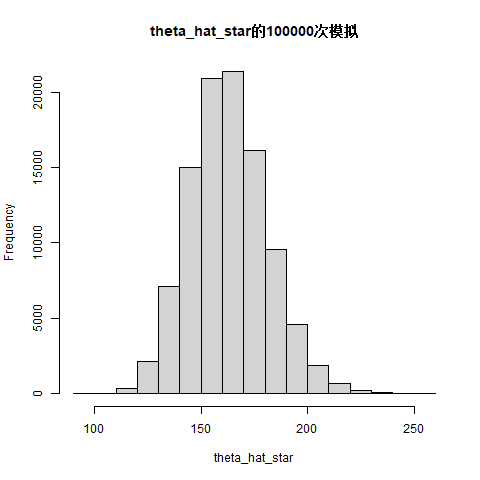
\includegraphics[scale=0.6]{bootstrap.png}
\end{minipage}
\\
这是$\hat{\theta}$的分布:\\
\begin{minipage}{0.5\textwidth}
    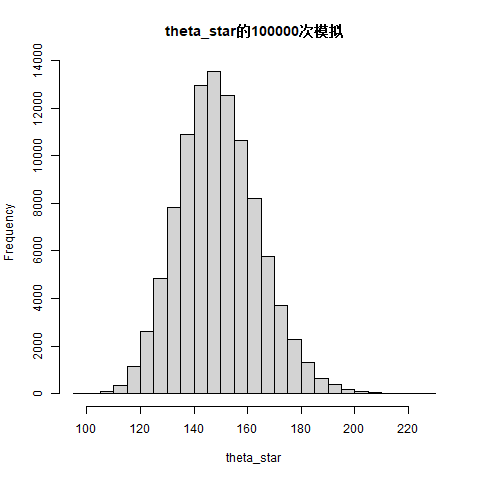
\includegraphics[scale=0.6]{bootstrap0.png}
\end{minipage}
\\可以看到二者的分布形状上比较接近,但方差有一定差异.
\\接下来,我做了10次模拟并比较二者的方差(实际上是样本方差),如下:\\
\begin{minipage}{0.5\textwidth}
    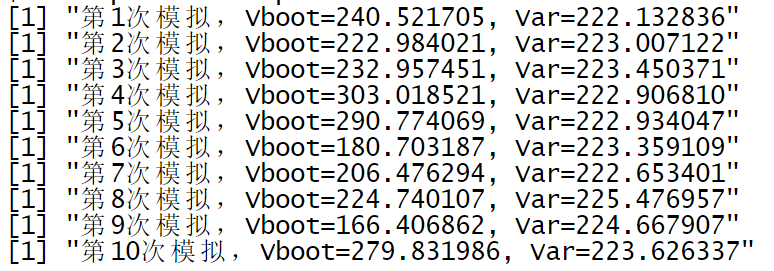
\includegraphics[scale=0.6]{bootstrap_data.png}
\end{minipage}
\\
可见$V_{boot}$具有对$Var(\hat{\theta})$的估计作用,但由于$V_{boot}$实际上只基于一组给定的样本,它的估计会产生较大的偏差.
\end{CJK}
\end{document}